\documentclass[]{article}

\usepackage{mathtools,mathrsfs,url,fancyhdr, graphicx,amsthm,tensor}

\renewcommand{\headrulewidth}{0pt}
\fancyhead[L]{}
\fancyhead[C]{
	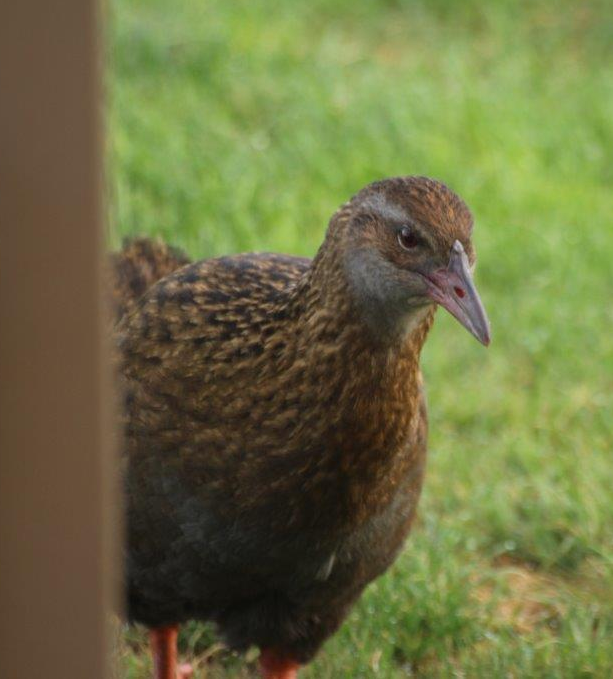
\includegraphics[width=2cm]{weka.png}
}
\graphicspath{ {images/} }

\newcommand{\Lagr}{\mathscr{L}}
\newcommand\numberthis{\addtocounter{equation}{1}\tag{\theequation}}
\newtheorem{theorem}{Theorem}
\pagestyle{plain}

\title{Introduction into General Relativity\\Assignment 3\\Problem 2\\Equations of Motion \& Stress Energy Tensor}
\author{Simon Crase}

\begin{document}

\maketitle
\thispagestyle{fancy}

 

\section{Scalar Field}
\subsection{Variation}
\begin{align*}
\text{We are given}&\\
S_M =& \int d^4x \, \sqrt{|g|} \, \left[\frac12 \, g^{\mu\nu} \, \partial_\mu \phi \, \partial_\nu \phi - V(\phi)\right] \numberthis \label{eq:action1}\\
\text{hence}&\\	
\delta_{\phi} S_M =& \delta_{\phi} \int d^4x \, \sqrt{|g|} \, \left[\frac{1}{2} \, g^{\mu\nu} \, \partial_\mu \phi \, \partial_\nu \phi - V(\phi)\right]\\
=&  \int d^4x \, \sqrt{|g|} \, \left[ \, g^{\mu\nu} \, \partial_\mu \phi \, \partial_\nu \delta \phi - V'(\phi) \delta \phi \right] \text{, since $g^{\mu\nu} \, \partial_\mu (\delta \phi) \, \partial_\nu \phi = g^{\mu\nu} \, \partial_\mu  \phi \, \partial_\nu \delta \phi$}\\
=&  \int d^4x \,  \, \left[ \underbrace{\big(\sqrt{|g|} \, g^{\mu\nu} \, \partial_\mu \phi \,\big) \big(\partial_\nu \delta \phi\big)}_\text{Integrate by parts} - \sqrt{|g|} V'(\phi) \delta \phi \right] \\
&\text{\{$\delta$ doesn't change integrand at boundary\}} \\
=& \int d^4x \big[ -\partial_\nu \big(\sqrt{|g|} g^{\mu\nu} \partial_\mu \phi\big) - \sqrt{|g|} V'(\phi)\big] \delta \phi \numberthis \label{eq:variation1}
\end{align*}
\subsection{Equations of motion}
Since $\delta_{\phi} S_M=0$ for all sufficiently small $\delta \phi$, (\ref{eq:variation1}) gives the following equation of motion.
\begin{align*}
-\partial_\nu \big(\sqrt{|g|} g^{\mu\nu} \partial_\mu \phi\big) - \sqrt{(|g|)} V'(\phi)=&0\\
\text{or}&\\
\frac{1}{\sqrt{(|g|)}} \partial_\nu \big(\sqrt{|g|} g^{\mu\nu} \partial_\mu \phi\big) =& -  V'(\phi)
\end{align*}
\subsection{Stress Tensor} \label{subseq:StressTensor}
In the Lecture Notes, \cite[Lecture III, Section 3]{akhmedev2016}, the Lagrangian, $\Lagr$, is defined by the expression $S_M = \int d^4x \, \sqrt{|g|} \Lagr$. Therefore, from \ref{eq:action1}. 
\begin{equation}
S_M = \int d^4x \, \sqrt{|g|} \underbrace{\left[\frac12 \, g^{\mu\nu} \, \partial_\mu \phi \, \partial_\nu \phi - V(\phi)\right]}_{\text{Lagrangian}\overset{\Delta}{=}\Lagr}
\end{equation}
So $\Lagr$ is given by
\begin{equation}
\Lagr=\frac12 \, g^{\mu\nu} \, \partial_\mu \phi \, \partial_\nu \phi - V(\phi)
\end{equation}
From the Lecture Notes \cite[(74)]{akhmedev2016}:
\begin{align}
T_{\mu\nu}&\overset{\Delta}{=}2 \frac{\partial \Lagr}{\partial g^{\mu\nu}} - \Lagr g_{\mu\nu} \nonumber \\
&=\frac{\partial [g^{\sigma\tau}\partial_\sigma \phi \partial_\tau \phi]}{\partial g^{\mu\nu}}-[\frac12 \, g^{\sigma\tau} \, \partial_\sigma \phi \, \partial_\tau \phi - V(\phi)] g_{\mu\nu} \nonumber \\
&=\frac{\partial [g^{\sigma\tau}\partial_\sigma \phi \partial_\tau \phi]}{\partial g^{\mu\nu}}-[\frac12 \, g^{\sigma\tau} \, \partial_\sigma \phi \, \partial_\tau \phi - V(\phi)] g_{\mu\nu} \nonumber\\
&=\frac{\partial g^{\sigma\tau}}{\partial g^{\mu\nu}}\partial_\sigma \phi \partial_\tau \phi-[\frac12 \, g^{\sigma\tau} \, \partial_\sigma \phi \, \partial_\tau \phi - V(\phi)] g_{\mu\nu} \nonumber \\
&=\partial_\mu \phi \partial_\nu \phi - \frac12 \, g_{\mu\nu} \, \partial_\sigma \phi \, \partial^\sigma \phi  + V(\phi) g_{\mu\nu} 
\end{align}

\section{Vector Potential}
\subsection{Variation}
We are given:
\begin{align*}
S_M =& \int d^4x \sqrt{|g|} \, F_{\mu\nu}\, F_{\alpha\beta} \, g^{\mu\alpha} \, g^{\nu\beta}\\
\text{whence}&\\
\delta_A S_M =& \delta_A \int d^4x \sqrt{|g|} \, F_{\mu\nu}\, F_{\alpha\beta} \, g^{\mu\alpha} \, g^{\nu\beta} \\
=&  \int d^4x \sqrt{|g|} \, F_{\mu\nu} \, g^{\mu\alpha} \, g^{\nu\beta} \, \delta_A F_{\alpha\beta} + \int d^4x \sqrt{|g|} \, (\delta_A F_{\mu\nu}) \, g^{\mu\alpha} \, g^{\nu\beta} \,  F_{\alpha\beta}\\
\text{We permute indices: }& (\mu\nu\alpha\beta)\rightarrow(\alpha\beta\mu\nu)\\
\delta_A S_M=& 2 \int d^4x \sqrt{|g|} \, F_{\mu\nu} \, g^{\mu\alpha} \, g^{\nu\beta} \, \delta_A F_{\alpha\beta} \\
=& 2 \int d^4x \sqrt{|g|} \, F_{\mu\nu} \, g^{\mu\alpha} \, g^{\nu\beta} \, \delta_A \big(\partial_\alpha A_\beta - \partial_\beta A_\alpha\big) \text{,  using \cite[(88)]{akhmedev2016}}\\
=& 4 \int d^4x \underbrace{\big(\sqrt{|g|} \, F_{\mu\nu} \, g^{\mu\alpha} \, g^{\nu\beta}\big) \, \delta \big(\partial_\alpha A_\beta \big)}_\text{Itegrate by parts}\\
=& -4 \int d^4x \, \partial_\alpha \big(\sqrt{|g|} \, F_{\mu\nu} \, g^{\mu\alpha} \, g^{\nu\beta} \,\big) \delta A_\beta\\
=& -4 \int d^4x \partial_\alpha \big(\sqrt{|g|} \, F^{\alpha\beta}  \,\big) \delta A_\beta
\end{align*}
\subsection{Equations of motion}
\begin{align*}
\partial_\alpha \big(\sqrt{|g|} \, F_{\mu\nu} \, g^{\mu\alpha} \, g^{\nu\beta} \,\big) &= 0 \numberthis \label{eq:eom} 
\end{align*}

\begin{theorem}
	Equation (\ref{eq:eom}) is equivalent to: $D_\alpha F^{\alpha\beta} = 0$.
\end{theorem}
\begin{proof}
	\begin{align*}
	D_\alpha F^{\alpha\beta} =& \partial_\alpha F^{\alpha\beta} \, + \, \Gamma^{\alpha}_{\rho\alpha}F^{\rho\beta}\,+\,\underbrace{\Gamma^\beta_{\rho\alpha}F^{\alpha\rho}}_{=0}\\
	&\text{\{Since $\Gamma$ is symmetric, and F antisymmetric\}} \\
	=& \partial_\alpha F^{\alpha\beta} \, + \, \Gamma^{\alpha}_{\rho\alpha}F^{\rho\beta}\\
	=& \partial_\alpha F^{\alpha\beta} \, + \, \frac{1}{2|g|}\big(\partial_\rho \, |g|\big)F^{\rho\beta} \numberthis \label{eq:eom_tem}
	\end{align*}
	Where we have used a well known result (e.g. \cite[equation (3.11)]{abs1965}), $\Gamma^{\alpha}_{\rho\alpha}=\frac{1}{2|g|}\big(\partial_\rho \, |g|\big)$.
	
	Now (\ref{eq:eom}) gives:
	\begin{align*}
	0 =& \partial_\alpha \big(\sqrt{|g|} \, F^{\alpha\beta} \big)\\
	=& \frac{1}{2\sqrt{|g|}} \big(\partial_\alpha g\big) F^{\alpha\beta} \, + \, \sqrt{|g|} \, \partial_\alpha F^{\alpha\beta}\\
	=& \sqrt{|g|} \big[\frac{1}{2|g|} \big(\partial_\alpha g\big) F^{\alpha\beta} \, + \, \, \partial_\alpha F^{\alpha\beta}\big]
	\end{align*}
	Comparing with (\ref{eq:eom_tem}),  $D_\alpha F^{\alpha\beta} = 0$.
\end{proof}
\subsection{Stress Tensor}
By a similar argument to Section \ref{subseq:StressTensor}:
\begin{equation}
\Lagr= F_{\mu\nu}\, F_{\alpha\beta} \, g^{\mu\alpha} \, g^{\nu\beta}.
\label {eq:a}
\end{equation}

and
\begin{align*}
T_{\mu\nu}&\overset{\Delta}{=}2 \frac{\partial \Lagr}{\partial g^{\mu\nu}} - \Lagr g_{\mu\nu}\\
&=2\frac{\partial F_{\sigma\tau}\, F_{\alpha\beta} \, g^{\sigma\alpha} \, g^{\tau\beta}}{\partial g^{\mu\nu}} - F_{\sigma\tau}\, F_{\alpha\beta} \, g^{\sigma\alpha} \, g^{\tau\beta} g_{\mu\nu} \\
&=2\frac{\partial F_{\sigma\tau}\, F_{\alpha\beta} \, g^{\sigma\alpha} \, g^{\tau\beta}}{\partial g^{\mu\nu}} - g_{\mu\nu} F^{\alpha\beta}\, F_{\alpha\beta} \numberthis \label {eg:stress}
\end{align*}
We can simplify the first term of (\ref{eg:stress}) by noting that the tensor $F$ does not depend on $g$, and that the components of $g$ are independent, so we can treat the partial derivative as a selection operator. Hence:
\begin{align*}
\frac{\partial \big(F_{\sigma\tau}\, F_{\alpha\beta} \, g^{\sigma\alpha} \, g^{\tau\beta}\big)}{\partial g^{\mu\nu}} =& \underbrace{F_{\mu\tau}\, F_{\nu\beta} \,  g^{\tau\beta}}_{\mu=\sigma \land \nu=\alpha} \: + \; \underbrace{F_{\sigma\mu}\, F_{\alpha\nu} \, g^{\sigma\alpha}}_{\mu=\tau \land \nu=\beta} \\
=& F_{\mu\tau}\, F\indices{_\nu^\tau} \; + \; \underbrace{F_{\mu\sigma}\, F_{\nu\alpha} g^{\sigma\alpha}}_\text{$F$ is antisymmetric, so if we swap indices twice, sign changes cancel} \\
=& F_{\mu\tau}\, F\indices{_\nu^\tau} \; + \; F_{\mu\sigma}\, F\indices{_\nu^\sigma} \\
=& 2 F_{\mu\tau}\, F\indices{_\nu^\tau} 
\end{align*}
Combining the last equation with (\ref{eg:stress}), we see:
$$T_{\mu\nu} = 4\big[F_{\mu\alpha} F\indices{_\nu^\alpha} - \frac{1}{4}g_{\mu\nu} F_{\alpha\beta} F^{\alpha\beta}\big]$$

\begin{thebibliography}{9}

\bibitem{akhmedev2016}
Emil T. Akhmedev,
\emph{Lectures on General Theory of Relativity},
2016,
\url{https://arxiv.org/pdf/1601.04996v6.pdf}.

\bibitem{abs1965}
Ronald Adler, Maurice Bazin, \& Menahem Schiffer,
\emph{Introduction to General Relativity},
McGraw-Hill Book Company, New York,
1965.
\end{thebibliography}

\end{document}
